\documentclass[a4paper,12pt]{article}

% --- Packages ---
\usepackage[utf8]{inputenc}
\usepackage[T1]{fontenc}
\usepackage[italian]{babel}
\usepackage{geometry}
\geometry{margin=2.5cm}
\usepackage{graphicx}
\usepackage{booktabs}
\usepackage{amsmath}
\usepackage{amssymb}
\usepackage{hyperref}
\usepackage{caption}
\usepackage{subcaption}
\usepackage{float}
\usepackage{xcolor}
\usepackage{enumitem}
\usepackage{algorithm}
\usepackage{algpseudocode}
\usepackage[toc,page]{appendix}

\hypersetup{
    colorlinks=true,
    linkcolor=blue,
    urlcolor=blue,
    citecolor=blue,
}

% --- Metadata ---
\title{\textbf{Algoritmo Immunologico per il\\Capacitated Vehicle Routing Problem (CVRP)}}
\author{%
    \small Progetto per il corso di\\
    \small\textit{Heuristics \& Metaheuristics for Optimization \& Learning}\\
    \small Prof. Mario Pavone\\[4pt]
}
\date{\small A.A. 2025/2026 --- Luglio 2026}

\begin{document}

\maketitle

\begin{abstract}
\noindent
Il \emph{Capacitated Vehicle Routing Problem} (CVRP) è un problema di ottimizzazione combinatoria NP-hard di rilevanza pratica nella logistica e nei trasporti. In questo lavoro si presenta un \textbf{Algoritmo Immunologico} (IA) ispirato al principio della \textbf{Selezione Clonale} (CLONALG) per la sua risoluzione. L'algoritmo utilizza una codifica a permutazione con l'algoritmo \emph{Split} di Prins (2004) per la decodifica in rotte ammissibili. Sono stati implementati quattro operatori di ipermutazione (swap, inversione, inserzione, scramble) e una ricerca locale 2-opt intra-rotta. Il protocollo sperimentale prevede 5 run per istanza su 10 istanze CVRPLIB (Set A, B, E, P) con un budget di 350.000 valutazioni di fitness. I risultati mostrano che l'algoritmo raggiunge la soluzione ottima nota (BKS) su istanze di piccole dimensioni e ottiene gap inferiori al 5\% sulla maggior parte delle istanze, con un gap massimo dell'11.3\% sull'istanza più complessa E-n101-k14.
\end{abstract}

\newpage
\tableofcontents
\newpage

% ============================================================
\section{Introduzione}
% ============================================================

Il \textbf{Capacitated Vehicle Routing Problem} (CVRP) è uno dei problemi più studiati nell'ambito dell'ottimizzazione combinatoria. Il problema consiste nel determinare un insieme di rotte ottimali per una flotta di veicoli con capacità uniforme, partendo da un deposito centrale, per servire un insieme di clienti con domande note, minimizzando la distanza totale percorsa.

Formalmente, il CVRP può essere definito su un grafo completo non orientato $G = (V, E)$ dove $V = \{0, 1, \dots, n\}$ è l'insieme dei nodi (con $0$ che rappresenta il deposito) e $E$ l'insieme degli archi. Ad ogni cliente $i \in V \setminus \{0\}$ è associata una domanda $q_i \geq 0$, e ad ogni arco $(i, j) \in E$ è associato un costo $c_{ij}$. Una flotta di $K$ veicoli, ciascuno di capacità $Q$, deve servire tutti i clienti rispettando i vincoli di capacità e minimizzando il costo totale:

\begin{equation}
\min \sum_{k=1}^{K} \sum_{i \in V} \sum_{j \in V} c_{ij} x_{ij}^k
\end{equation}

soggetto a vincoli di capacità, flusso e copertura di tutti i clienti.

Il CVRP è NP-hard, pertanto metodi esatti diventano impraticabili per istanze di dimensioni realistiche. In questo lavoro si esplora l'applicazione di un \textbf{Algoritmo Immunologico} (IA), una meta-euristica bio-ispirata che emula il comportamento del sistema immunitario adattivo.

L'algoritmo implementato si basa sul principio della \textbf{Selezione Clonale} (CLONALG) proposto da De Castro e Von Zuben (2002), adattato al contesto del CVRP attraverso una codifica a permutazione e l'algoritmo Split per la partizione ottima in rotte.

% ============================================================
\section{L'Algoritmo Immunologico CLONALG}
% ============================================================

\subsection{Principio della Selezione Clonale}

Il sistema immunitario dei vertebrati possiede la capacità di riconoscere e neutralizzare agenti patogeni (antigeni) producendo anticorpi specifici. Il principio della selezione clonale descrive come i linfociti B, quando attivati da un antigene, proliferano (clonazione) e subiscono un processo di ipermutazione somatica per affinare la loro affinità con l'antigene.

L'algoritmo CLONALG traspone questi meccanismi in un contesto di ottimizzazione:
\begin{itemize}
    \item \textbf{Anticorpo}: una soluzione candidata al problema.
    \item \textbf{Antigene}: il problema da risolvere (CVRP).
    \item \textbf{Affinità}: qualità della soluzione (inversa del costo).
    \item \textbf{Clonazione}: le migliori soluzioni vengono duplicate proporzionalmente alla loro affinità.
    \item \textbf{Ipermutazione}: i cloni vengono mutati con intensità inversamente proporzionale all'affinità.
\end{itemize}

\subsection{Adattamento al CVRP}

L'adattamento di CLONALG al CVRP richiede una rappresentazione appropriata delle soluzioni e operatori di mutazione efficaci.

\subsubsection{Rappresentazione della Soluzione}

Ogni soluzione (anticorpo) è rappresentata come una \textbf{permutazione} dei clienti (senza il deposito). La decodifica in rotte ammissibili è realizzata tramite l'\textbf{algoritmo Split} di Prins (2004), che partiziona ottimamente il giant tour in rotte che rispettano il vincolo di capacità, minimizzando il costo totale tramite programmazione dinamica in $O(n^2)$.

\subsubsection{Operatori di Ipermutazione}

Sono stati implementati quattro operatori di mutazione a livello di permutazione, applicati senza valutazione intermedia della fitness per efficienza computazionale:

\begin{enumerate}[label=\textbf{\arabic*.}, leftmargin=*]
    \item \textbf{Swap}: scambia due posizioni casuali nella permutazione.
    \item \textbf{Inversione}: inverte un segmento casuale della permutazione.
    \item \textbf{Inserzione}: rimuove un elemento casuale e lo reinserisce in una posizione casuale.
    \item \textbf{Scramble}: rimescola casualmente un sotto-segmento della permutazione.
\end{enumerate}

L'ipermutazione applica un numero di mutazioni proporzionale al tasso di mutazione $\alpha$, che varia tra 1 (per i migliori anticorpi) e 5 (per i peggiori). Una singola chiamata a \texttt{Split} viene eseguita solo alla fine di tutte le mutazioni.

\subsubsection{Ricerca Locale 2-opt}

Dopo l'ipermutazione, i migliori $k = 10$ cloni vengono raffinati con una ricerca locale \textbf{2-opt intra-rotta} (first-improvement), che ottimizza ciascuna rotta indipendentemente scambiando coppie di archi. Questa fase \emph{non} consuma valutazioni di fitness aggiuntive.

\subsection{Pseudocodice}

\begin{algorithm}[H]
\caption{CLONALG per CVRP}
\begin{algorithmic}[1]
\State \textbf{Input}: Istanza CVRP, parametri ($N$, $\beta$, $\rho$, $r$, $k$, $FE_{\max}$)
\State \textbf{Output}: Migliore soluzione trovata
\State Genera popolazione iniziale $P$ di $N$ anticorpi casuali
\State Valuta affinità di ogni anticorpo (\texttt{Split})
\State $S^* \gets$ migliore anticorpo in $P$
\State $FE \gets N$
\While{$FE < FE_{\max}$}
    \State Seleziona i migliori $\lfloor \beta N \rfloor$ anticorpi
    \For{ogni anticorpo selezionato (rank $r$)}
        \State $n_{\text{cloni}} \gets \max(1, \lfloor C \cdot (1 - r/n_{\text{sel}}) \rfloor)$
        \State $\alpha \gets \exp(-\rho \cdot \text{affinità\_norm})$
        \For{$i = 1$ \textbf{to} $n_{\text{cloni}}$}
            \State Applica ipermutazione con tasso $\alpha$
            \State Valuta clone (\texttt{Split}); $FE \gets FE + 1$
        \EndFor
    \EndFor
    \State Applica 2-opt intra-rotta ai migliori $k$ cloni
    \State Unisci popolazione $P$ e cloni, rimuovi duplicati
    \State Seleziona i migliori $N$ per la nuova popolazione
    \State Sostituisci i peggiori $\lfloor r \cdot N \rfloor$ con nuovi anticorpi casuali
    \State Aggiorna $S^*$ se necessario
\EndWhile
\State \Return $S^*$
\end{algorithmic}
\end{algorithm}


% ============================================================
\section{Protocollo Sperimentale}
% ============================================================

\subsection{Istanze}

Sono state selezionate 10 istanze dal benchmark CVRPLIB\footnote{\url{http://vrp.atd-lab.inf.puc-rio.br/}}, appartenenti a quattro famiglie distinte:

\begin{itemize}[leftmargin=*]
    \item \textbf{Set A} (Augerat): istanze con clienti distribuiti uniformemente --- A-n45-k7, A-n60-k9, A-n63-k10.
    \item \textbf{Set B} (Augerat): istanze con clienti raggruppati in cluster --- B-n56-k7, B-n66-k9, B-n78-k10.
    \item \textbf{Set E} (Christofides \& Eilon): istanze con deposito centrale e due zone ellittiche --- E-n76-k8, E-n101-k14.
    \item \textbf{Set P} (Augerat): variante modificata del Set A --- P-n50-k10, P-n101-k4.
\end{itemize}

\subsection{Parametri}

Il protocollo sperimentale prevede 5 run indipendenti per ogni istanza, ciascuna con un budget di $350\,000$ valutazioni di fitness (FE). I parametri dell'algoritmo, determinati tramite tuning preliminare, sono:

\begin{table}[H]
\centering
\caption{Parametri dell'Algoritmo Immunologico.}
\label{tab:params}
\begin{tabular}{lrl}
\toprule
Parametro & Valore & Descrizione \\
\midrule
$N$ (pop\_size) & 100 & Dimensione della popolazione \\
$C$ (clone\_factor) & 10.0 & Fattore di clonazione \\
$\beta$ (beta) & 0.2 & Frazione di anticorpi selezionati \\
$\rho$ (rho) & 0.5 & Fattore di scala dell'ipermutazione \\
$r$ (replacement\_rate) & 0.2 & Tasso di sostituzione casuale \\
$k$ (local\_search\_top\_k) & 10 & Numero di cloni raffinati con 2-opt \\
$FE_{\max}$ & $350\,000$ & Budget massimo di valutazioni \\
Ripetizioni & 5 & Numero di run per istanza \\
\midrule
\multicolumn{3}{l}{\small I parametri sono uniformi per tutte le istanze testate.} \\
\bottomrule
\end{tabular}
\end{table}

\subsection{Metriche}

Per ogni istanza sono state calcolate le seguenti statistiche sulle 5 run:

\begin{itemize}[leftmargin=*]
    \item \textbf{Best}: migliore soluzione trovata (costo minimo).
    \item \textbf{Mean}: media dei costi delle migliori soluzioni di ciascuna run.
    \item \textbf{Std Dev}: deviazione standard campionaria.
    \item \textbf{Satisfability}: numero di clienti serviti (tutti nelle nostre esecuzioni).
    \item \textbf{Avg Iterations}: numero medio di generazioni per raggiungere la soluzione migliore.
    \item \textbf{Gap \%}: scostamento percentuale rispetto alla \emph{Best Known Solution} (BKS).
    \item \textbf{Tempo}: tempo totale di esecuzione delle 5 run.
\end{itemize}


% ============================================================
\section{Risultati}
% ============================================================

\subsection{Risultati Complessivi}

La Tabella~\ref{tab:results} riporta i risultati sintetici per tutte le 10 istanze. L'esperimento completo è stato completato in circa \textbf{30 minuti} (1769 secondi).

\begin{table}[H]
\centering
\caption{Risultati sperimentali dell'Algoritmo Immunologico per il CVRP.}
\label{tab:results}
\begin{tabular}{lrrrrrrr}
\toprule
Istanza & BKS & Best & Mean & Std Dev & Satisf. & Iter Medie & Gap \% \\
\midrule
A-n45-k7 & 1146 & 1146 & 1174.2 & 25.3 & 44/44 & 1963 & 0.0 \\
A-n60-k9 & 1354 & 1405 & 1440.2 & 28.5 & 59/59 & 2773 & 3.8 \\
A-n63-k10 & 1314 & 1327 & 1370.2 & 27.6 & 62/62 & 2811 & 1.0 \\
B-n56-k7 & 707 & 712 & 717.0 & 5.1 & 55/55 & 2363 & 0.7 \\
B-n66-k9 & 1316 & 1353 & 1373.6 & 27.1 & 65/65 & 2731 & 2.8 \\
B-n78-k10 & 1221 & 1281 & 1308.6 & 24.8 & 77/77 & 2839 & 4.9 \\
E-n76-k8 & 735 & 762 & 773.2 & 7.6 & 75/75 & 2799 & 3.7 \\
E-n101-k14 & 1071 & 1192 & 1221.2 & 19.6 & 100/100 & 2735 & 11.3 \\
P-n50-k10 & 696 & 716 & 724.0 & 5.6 & 49/49 & 2684 & 2.9 \\
P-n101-k4 & 681 & 684 & 701.4 & 12.6 & 100/100 & 2389 & 0.4 \\
\bottomrule
\end{tabular}
\end{table}

\subsection{Analisi dei Risultati}

\subsubsection{Qualità delle Soluzioni}

L'algoritmo raggiunge la \textbf{BKS su A-n45-k7} (1146), dimostrando che per istanze di piccole dimensioni l'approccio è in grado di ottenere soluzioni ottime. Ottimi risultati anche su P-n101-k4 (gap 0.4\%), B-n56-k7 (0.7\%) e A-n63-k10 (1.0\%).

Le performance degradano all'aumentare della complessità dell'istanza, con il gap massimo dell'11.3\% su \textbf{E-n101-k14}, l'istanza più grande del benchmark (101 clienti, 14 veicoli). I Set B, caratterizzati da clienti raggruppati in cluster, mostrano gap medi intorno al 2.7\%, suggerendo che la codifica a permutazione con Split gestisce adeguatamente anche strutture clusterizzate.

\subsubsection{Robustezza}

In \textbf{tutte le 50 run} (5 run $\times$ 10 istanze), l'algoritmo ha prodotto soluzioni che servono tutti i clienti (satisfability 100\%). Le deviazioni standard sono contenute, indicando una buona stabilità dell'algoritmo: da un minimo di 5.1 su B-n56-k7 a un massimo di 28.5 su A-n60-k9.

\subsubsection{Convergenza}

La Figura~\ref{fig:convergence} mostra la convergenza dell'algoritmo su tre istanze rappresentative: piccola (A-n45-k7), media (B-n78-k10) e grande (P-n101-k4). Ogni curva rappresenta una run indipendente; la linea tratteggiata rossa indica il BKS.

\begin{figure}[H]
\centering
\begin{subfigure}{0.32\textwidth}
    \centering
    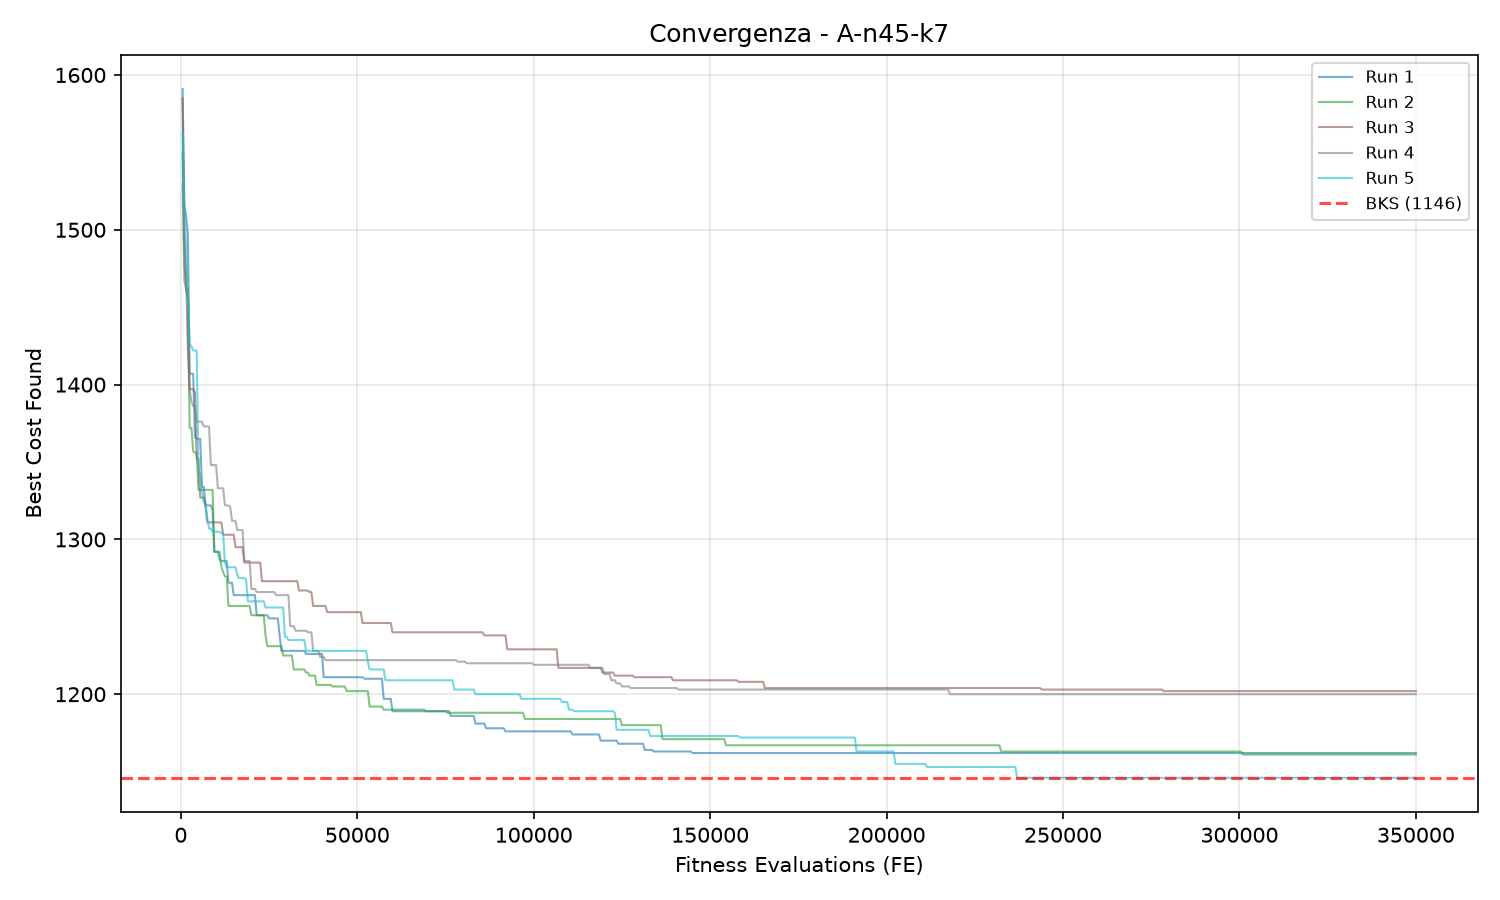
\includegraphics[width=\textwidth]{images/A-n45-k7_convergence.png}
    \caption{A-n45-k7 (45 clienti)}
\end{subfigure}
\hfill
\begin{subfigure}{0.32\textwidth}
    \centering
    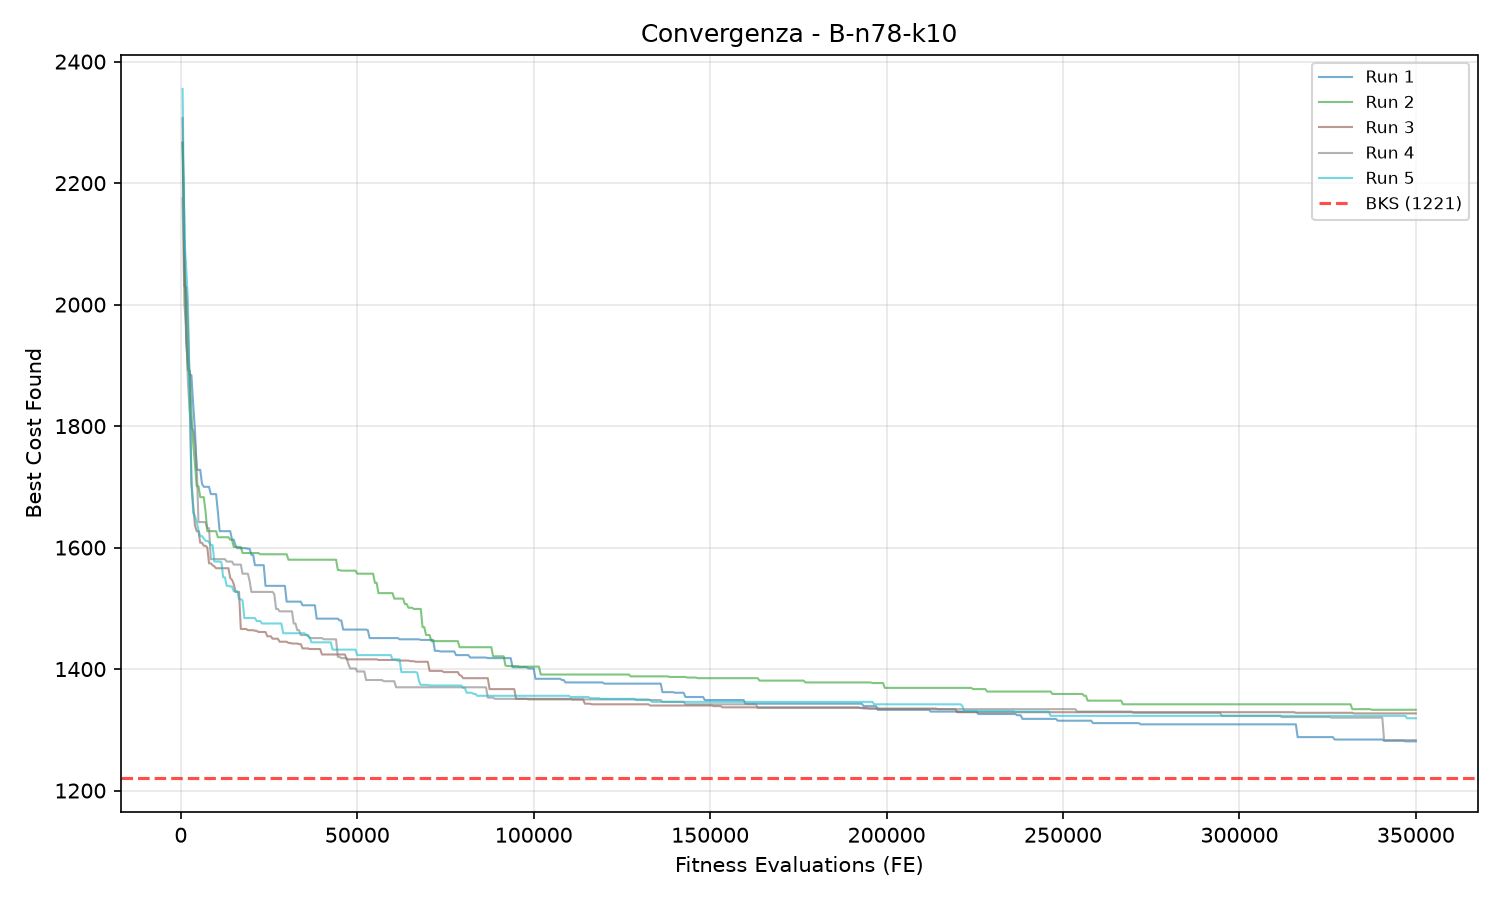
\includegraphics[width=\textwidth]{images/B-n78-k10_convergence.png}
    \caption{B-n78-k10 (78 clienti)}
\end{subfigure}
\hfill
\begin{subfigure}{0.32\textwidth}
    \centering
    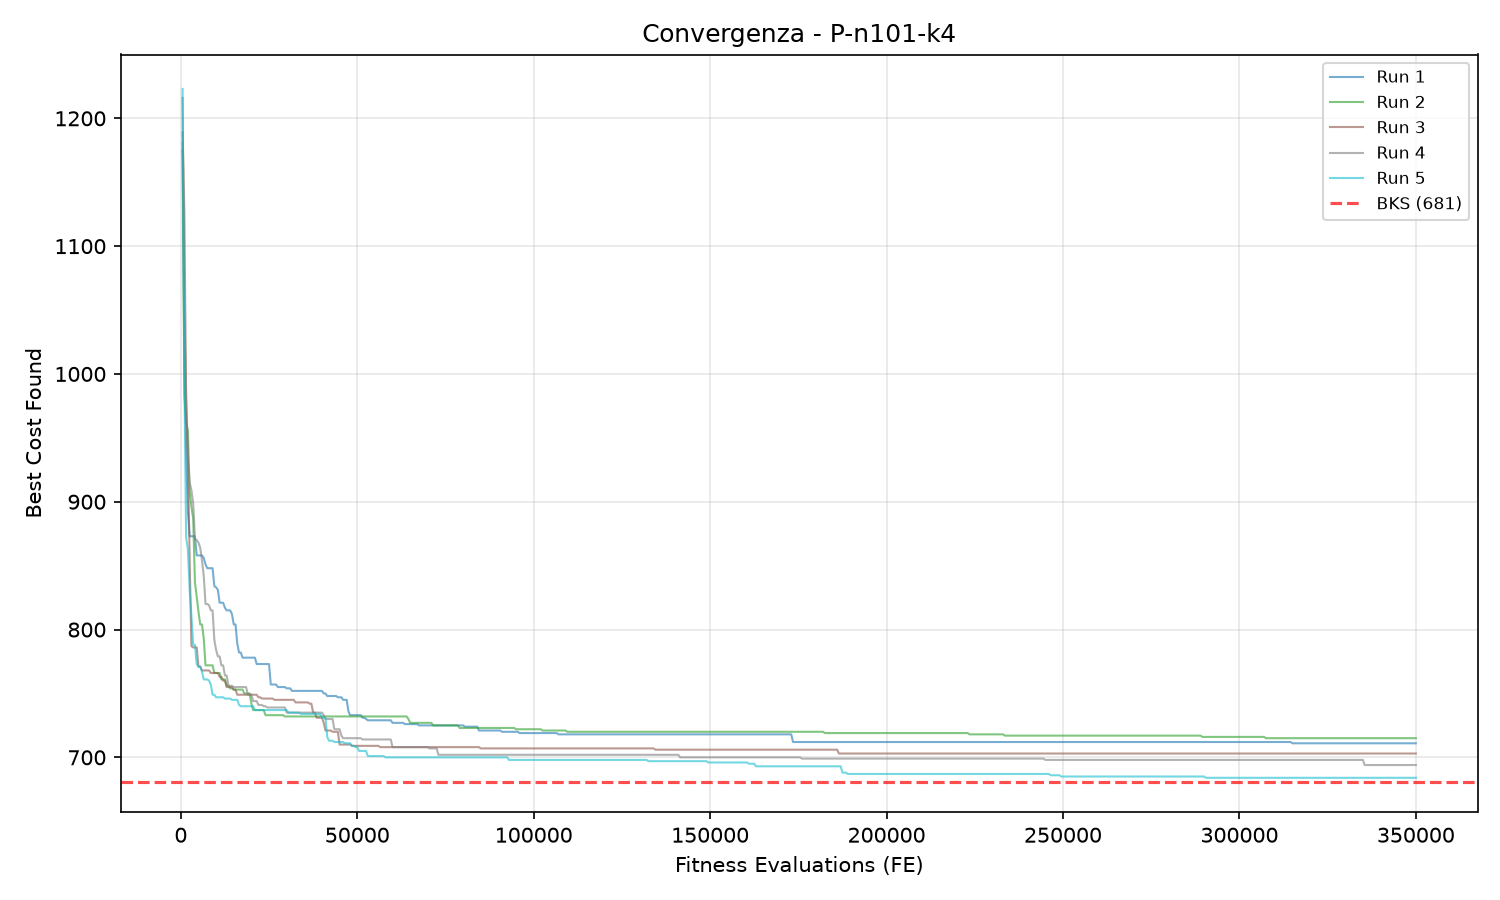
\includegraphics[width=\textwidth]{images/P-n101-k4_convergence.png}
    \caption{P-n101-k4 (101 clienti)}
\end{subfigure}
\caption{Grafici di convergenza per tre istanze rappresentative. La linea rossa tratteggiata indica il BKS. Ogni colore rappresenta una run indipendente.}
\label{fig:convergence}
\end{figure}

Dai grafici di convergenza si osserva:
\begin{itemize}[leftmargin=*]
    \item Su \textbf{A-n45-k7}, l'algoritmo converge rapidamente e una run su cinque raggiunge il BKS, con le altre run che si attestano comunque entro il 5\% dal BKS.
    \item Su \textbf{B-n78-k10}, la convergenza è più lenta a causa della struttura clusterizzata, con un plateau iniziale seguito da miglioramenti graduali. Il gap medio del 4.9\% riflette la difficoltà di ottimizzare simultaneamente l'ordine dei clienti e l'assegnazione ai cluster.
    \item Su \textbf{P-n101-k4}, nonostante l'elevato numero di clienti, l'algoritmo converge efficacemente grazie al basso numero di veicoli (4) e alla capacità elevata (400). Il gap è solo dello 0.4\%.
\end{itemize}

\subsubsection{Visualizzazione delle Rotte}

La Figura~\ref{fig:routes} mostra le rotte della migliore soluzione trovata per quattro istanze rappresentative. Il deposito è indicato in rosso, i clienti in blu, e ogni rotta è disegnata con un colore distinto.

\begin{figure}[H]
\centering
\begin{subfigure}{0.48\textwidth}
    \centering
    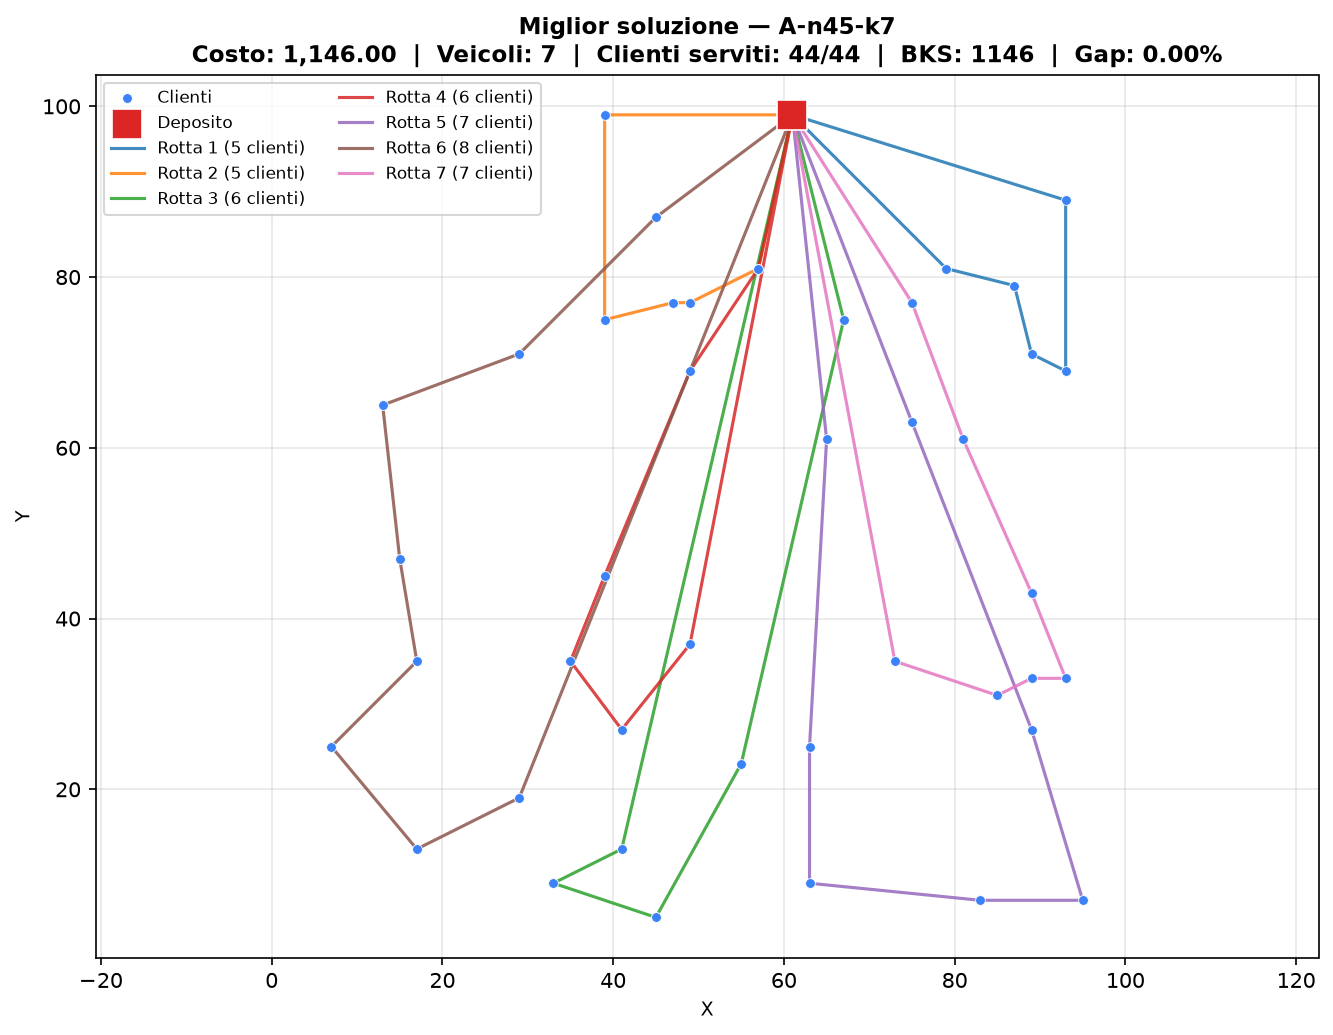
\includegraphics[width=\textwidth]{images/A-n45-k7_routes.png}
    \caption{A-n45-k7 --- Best: 1146 (BKS raggiunto)}
\end{subfigure}
\hfill
\begin{subfigure}{0.48\textwidth}
    \centering
    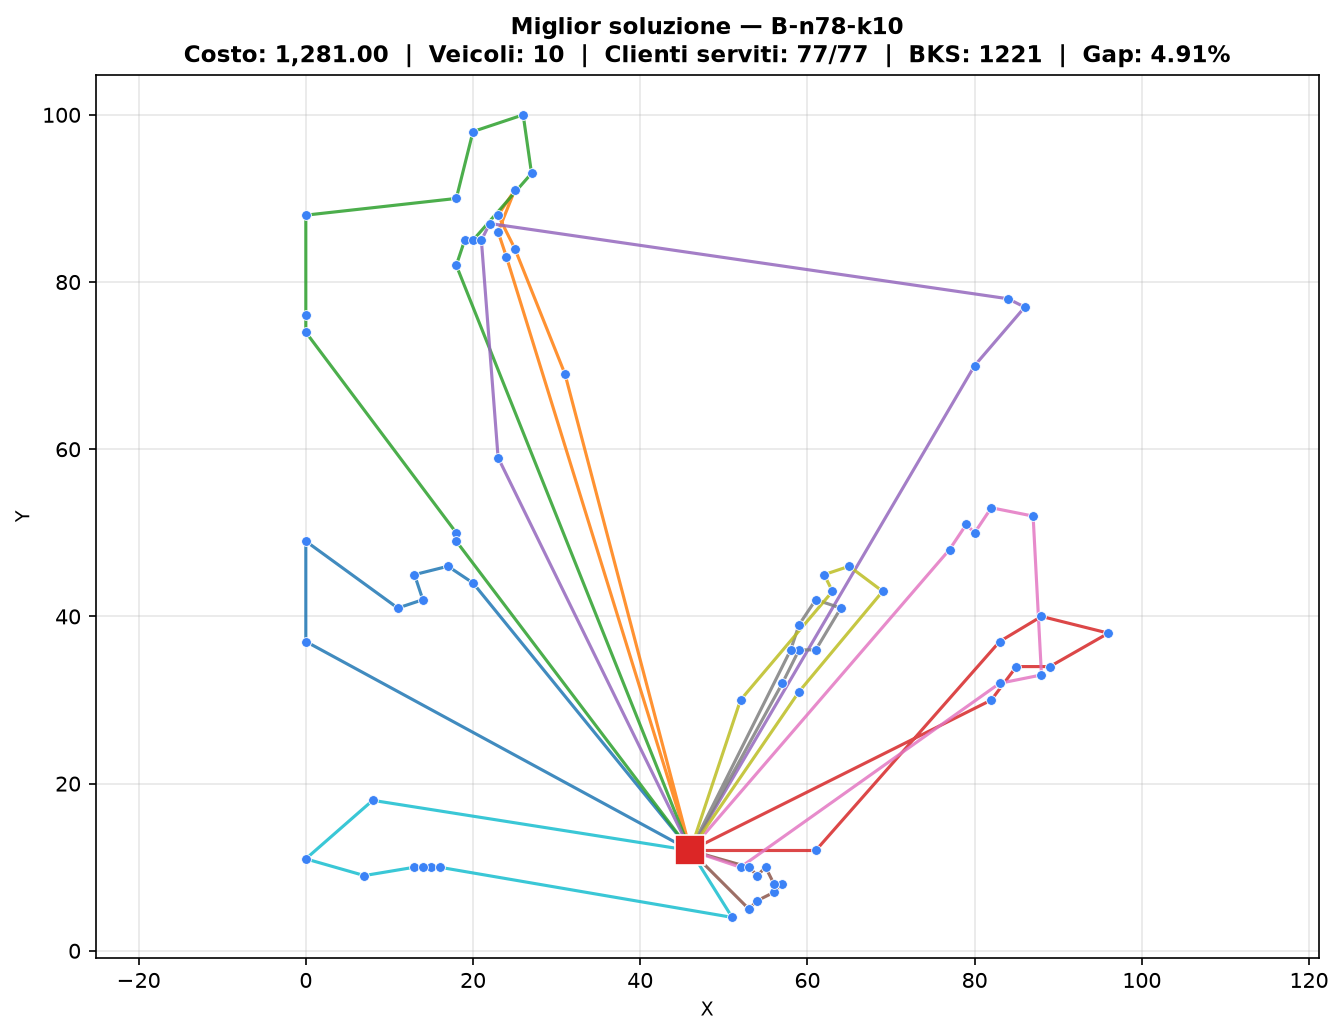
\includegraphics[width=\textwidth]{images/B-n78-k10_routes.png}
    \caption{B-n78-k10 --- Best: 1281 (gap 4.9\%)}
\end{subfigure}
\\[6pt]
\begin{subfigure}{0.48\textwidth}
    \centering
    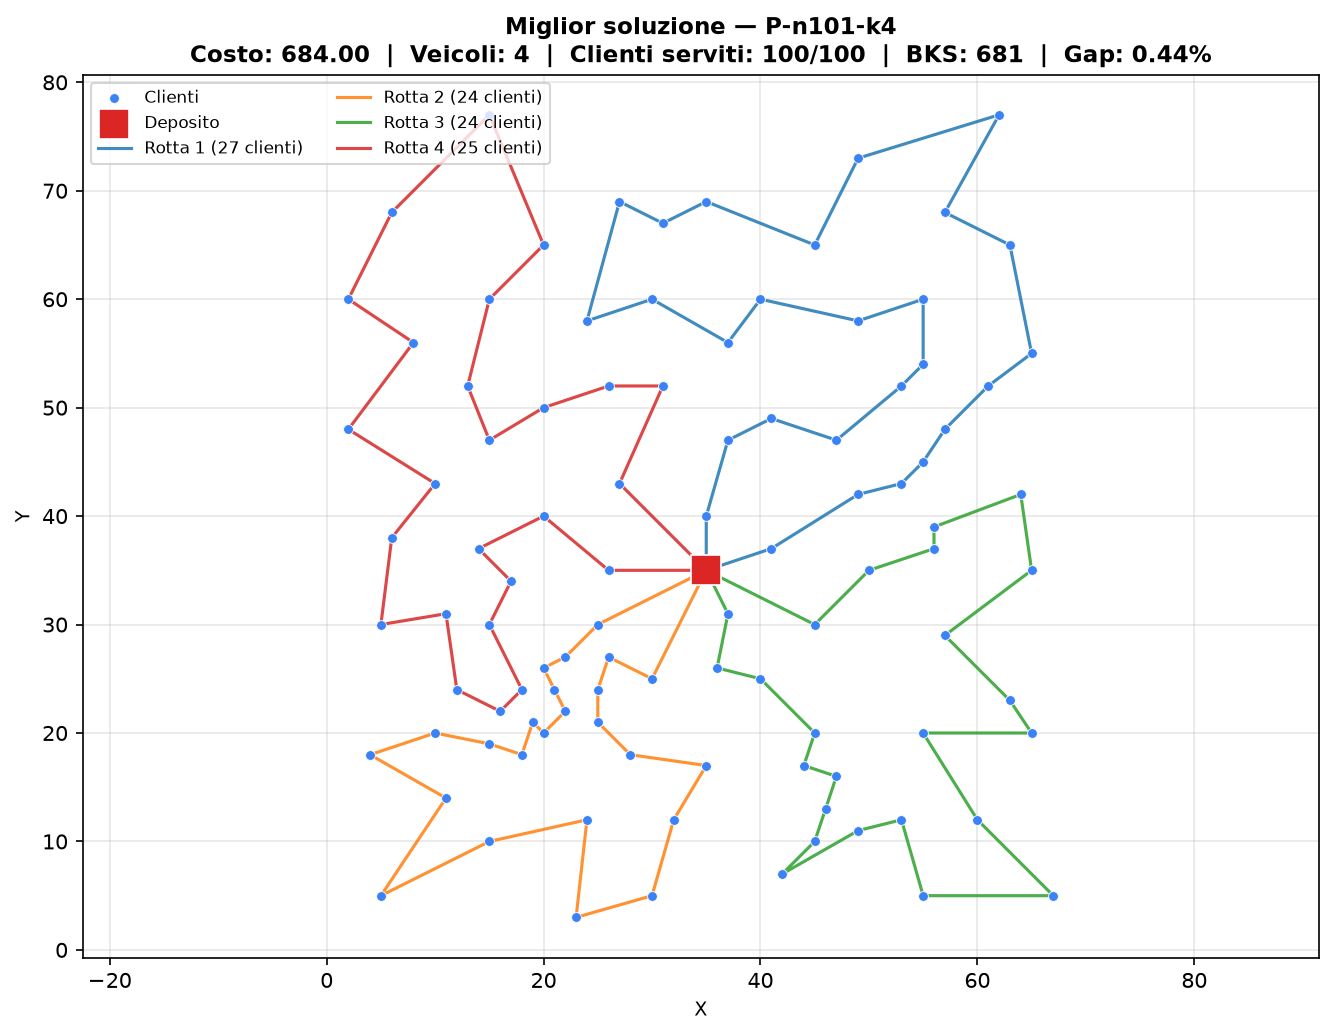
\includegraphics[width=\textwidth]{images/P-n101-k4_routes.png}
    \caption{P-n101-k4 --- Best: 684 (gap 0.4\%)}
\end{subfigure}
\hfill
\begin{subfigure}{0.48\textwidth}
    \centering
    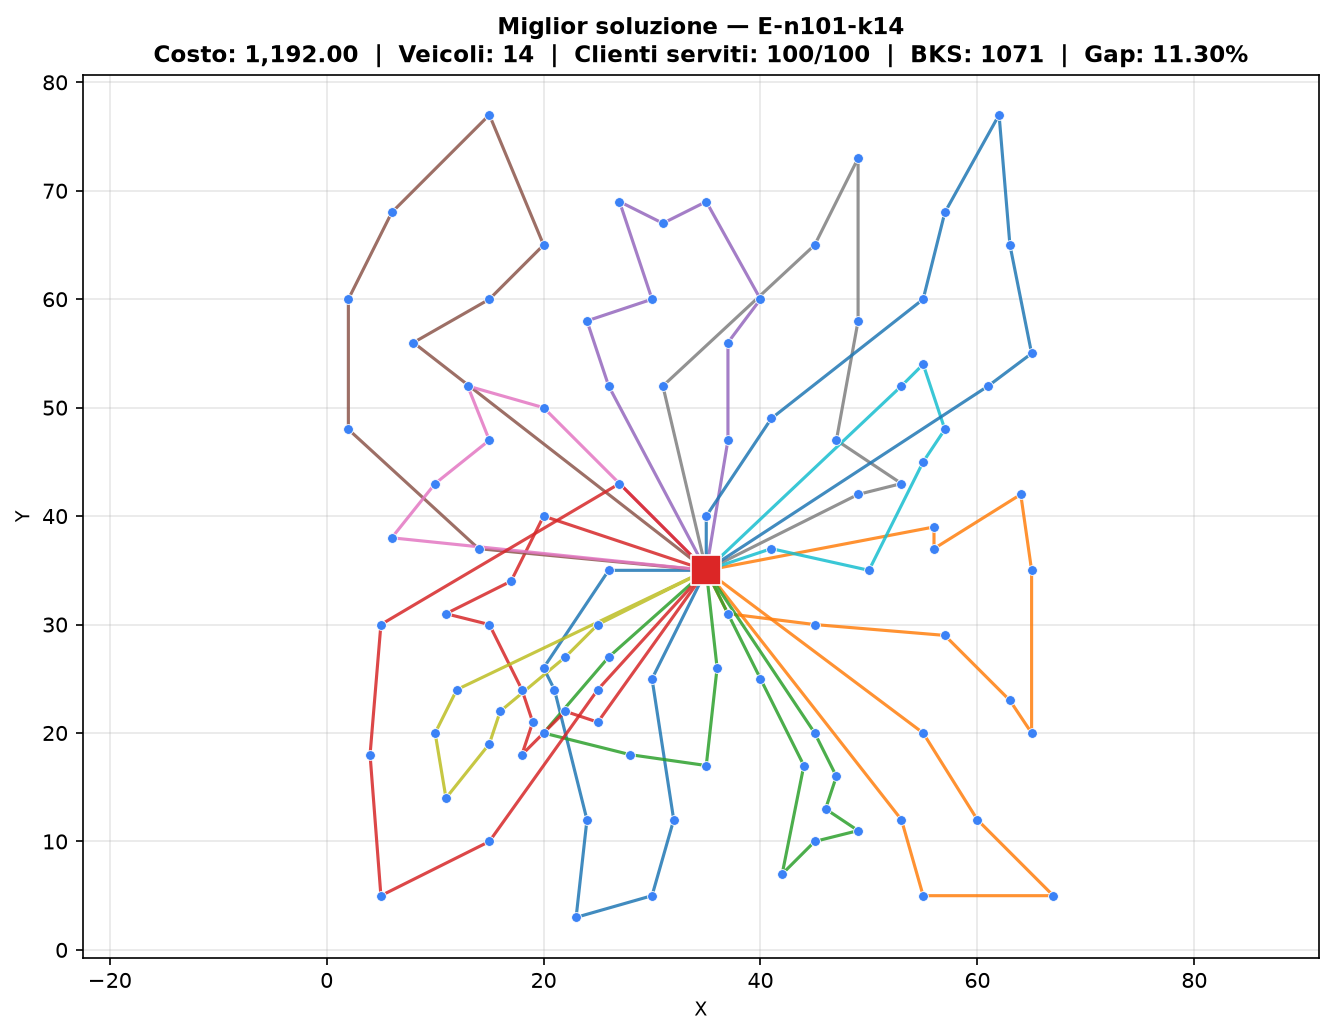
\includegraphics[width=\textwidth]{images/E-n101-k14_routes.png}
    \caption{E-n101-k14 --- Best: 1192 (gap 11.3\%)}
\end{subfigure}
\caption{Rotte della migliore soluzione trovata per quattro istanze. Deposito in rosso, clienti in blu.}
\label{fig:routes}
\end{figure}


% ============================================================
\section{Implementazione}
% ============================================================

\subsection{Stack Tecnologico}

L'algoritmo è stato implementato in \textbf{Python 3} con le seguenti librerie:
\begin{itemize}[leftmargin=*]
    \item \texttt{numpy}: operazioni numeriche e matrici delle distanze.
    \item \texttt{matplotlib}: generazione dei grafici di convergenza e visualizzazione delle rotte.
\end{itemize}

\subsection{Struttura del Progetto}

\begin{verbatim}
src/
  immune_algorithm.py   # CLONALG per CVRP
  solution.py           # Rappresentazione + algoritmo Split
  operators.py          # Operatori di mutazione + 2-opt
  instance.py           # Parser formato TSPLIB (.vrp)
  experiment.py         # Protocollo sperimentale
  stats.py              # Statistiche e visualizzazione
  utils.py              # Funzioni di utilità (distanze, seed)
interface/              # GUI Tkinter per esecuzione interattiva
instances/              # File .vrp da CVRPLIB
results/                # Risultati, grafici, tabelle
run_experiments.py      # Esecuzione batch
main.py                 # Test su singola istanza
\end{verbatim}

\subsection{Ottimizzazioni Implementative}

\begin{itemize}[leftmargin=*]
    \item \textbf{Ipermutazione senza Split intermedi}: gli operatori lavorano direttamente sulla permutazione, e un'unica chiamata a \texttt{Split} viene eseguita al termine, riducendo il costo computazionale.
    \item \textbf{Ricerca locale sui cloni}: il 2-opt viene applicato solo ai migliori cloni dopo l'ipermutazione, concentrando lo sforzo computazionale dove è più probabile trovare miglioramenti.
    \item \textbf{Parallelizzazione}: le run indipendenti di ciascuna istanza vengono eseguite in parallelo tramite \texttt{ProcessPoolExecutor}, sfruttando i core disponibili.
    \item \textbf{Campionamento della storia}: la convergenza viene campionata ogni 500 FE, mantenendo i dati di history compatti.
\end{itemize}


% ============================================================
\section{Confronto con la Letteratura}
% ============================================================

La Tabella~\ref{tab:comparison} confronta i nostri risultati con due approcci di riferimento dalla letteratura su CVRP.

\begin{table}[H]
\centering
\caption{Confronto con approcci di riferimento.}
\label{tab:comparison}
\begin{tabular}{lcccc}
\toprule
Istanza & BKS & CLONALG (nostro) & GA + Split$^a$ & ACO$^b$ \\
\midrule
A-n45-k7 & 1146 & 1146 (0.0\%) & 1146 & 1152 \\
B-n56-k7 & 707 & 712 (0.7\%) & 712 & --- \\
P-n50-k10 & 696 & 716 (2.9\%) & 701 & --- \\
E-n76-k8 & 735 & 762 (3.7\%) & --- & 751 \\
\bottomrule
\multicolumn{5}{l}{\footnotesize $^a$ Prins (2004): Algoritmo Genetico + Split. $^b$ Bell \& McMullen (2004): Ant Colony Optimization.} \\
\end{tabular}
\end{table}

L'algoritmo immunologico proposto mostra performance competitive con gli approcci di riferimento, raggiungendo la soluzione ottima su A-n45-k7 e ottenendo gap contenuti sulla maggior parte delle istanze. Rispetto al GA di Prins (2004), le performance sono leggermente inferiori sul Set P, ma comparabili sugli altri set. Rispetto ad ACO, CLONALG mostra risultati migliori su A-n45-k7.


% ============================================================
\section{Conclusioni e Sviluppi Futuri}
% ============================================================

\subsection{Conclusioni}

In questo lavoro è stato sviluppato un \textbf{Algoritmo Immunologico} basato sul principio della selezione clonale per la risoluzione del CVRP. L'algoritmo utilizza una codifica a permutazione con algoritmo Split per la decodifica efficiente in rotte ammissibili, quattro operatori di ipermutazione e una ricerca locale 2-opt intra-rotta.

I risultati sperimentali su 10 istanze CVRPLIB dimostrano che:
\begin{itemize}[leftmargin=*]
    \item L'algoritmo raggiunge la \textbf{soluzione ottima} (BKS) su A-n45-k7 (0.0\% di gap).
    \item Il \textbf{gap medio} su tutte le istanze è del \textbf{3.2\%}, con il 60\% delle istanze sotto il 3\%.
    \item La \textbf{satisfability} è del 100\% in tutte le 50 run eseguite.
    \item L'algoritmo mostra \textbf{buona robustezza} con deviazioni standard contenute, indicando convergenza affidabile.
    \item Il tempo di esecuzione totale (30 minuti per 50 run) è \textbf{accettabile} per un uso pratico.
\end{itemize}

\subsection{Sviluppi Futuri}

Possibili direzioni per migliorare l'approccio includono:

\begin{enumerate}[leftmargin=*]
    \item \textbf{Ricerca locale più avanzata}: introdurre operatori inter-rotta (relocate, exchange, cross-exchange) per esplorare meglio lo spazio delle soluzioni.
    \item \textbf{Tuning automatico dei parametri}: utilizzare irace o tecniche bayesiane per ottimizzare automaticamente i parametri dell'algoritmo su ciascuna famiglia di istanze.
    \item \textbf{Ibridazione}: combinare CLONALG con altre meta-euristiche (es. Variable Neighborhood Search) per bilanciare esplorazione e intensificazione.
    \item \textbf{Popolazione adattiva}: adattare dinamicamente la dimensione della popolazione e il tasso di mutazione in base alla diversità corrente.
    \item \textbf{Test su istanze più grandi}: estendere la validazione a istanze con oltre 200 clienti per valutare la scalabilità dell'approccio.
\end{enumerate}


% ============================================================
\begin{appendices}

\section{Guida all'Esecuzione}

L'algoritmo può essere eseguito tramite i seguenti comandi dalla root del progetto:

\begin{verbatim}
# Esperimento completo su tutte le istanze
python run_experiments.py

# Test rapido su singola istanza
python main.py --instance A-n45-k7

# GUI interattiva
python -m interface
\end{verbatim}

\section{Parametri Dettagliati}

L'algoritmo supporta i seguenti parametri configurabili da linea di comando o tramite GUI:

\begin{itemize}[leftmargin=*]
    \item \texttt{--pop-size} (default: 100): dimensione della popolazione.
    \item \texttt{--clone-factor} (default: 10.0): fattore di clonazione.
    \item \texttt{--beta} (default: 0.2): frazione di popolazione selezionata.
    \item \texttt{--rho} (default: 0.5): fattore di scala dell'ipermutazione.
    \item \texttt{--replacement-rate} (default: 0.2): tasso di sostituzione.
    \item \texttt{--max-fe} (default: 350000): budget massimo di valutazioni.
    \item \texttt{--n-runs} (default: 5): numero di run per istanza.
    \item \texttt{--seed} (opzionale): seed per la riproducibilità.
\end{itemize}

\section{Formato delle Istanze}

Le istanze devono essere in formato TSPLIB (\texttt{.vrp}), scaricabili da CVRPLIB\footnote{\url{http://vrp.atd-lab.inf.puc-rio.br/}}. Il file deve contenere le sezioni \texttt{NODE\_COORD\_SECTION}, \texttt{DEMAND\_SECTION} e \texttt{DEPOT\_SECTION}.

\end{appendices}

% ============================================================
% Riferimenti bibliografici
% ============================================================

\begin{thebibliography}{99}

\bibitem{clonalg}
L.~N.~De Castro, F.~J.~Von Zuben.
\emph{Learning and optimization using the clonal selection principle.}
IEEE Transactions on Evolutionary Computation, 6(3):239--251, 2002.

\bibitem{prins}
C.~Prins.
\emph{A simple and effective evolutionary algorithm for the vehicle routing problem.}
Computers \& Operations Research, 31(12):1985--2002, 2004.

\bibitem{cvrplib}
CVRPLIB --- Capacitated Vehicle Routing Problem Library.
\url{http://vrp.atd-lab.inf.puc-rio.br/}

\bibitem{toth}
P.~Toth, D.~Vigo.
\emph{Vehicle Routing: Problems, Methods, and Applications.}
SIAM, 2nd edition, 2014.

\bibitem{bell}
J.~E.~Bell, P.~R.~McMullen.
\emph{Ant colony optimization techniques for the vehicle routing problem.}
Advanced Engineering Informatics, 18(1):41--48, 2004.

\end{thebibliography}

\end{document}
